\documentclass[twocolumn,10pt,a4paper]{article}

\usepackage[margin=1.8cm]{geometry}
\usepackage{amsmath,amssymb,amsfonts,amsthm}
\usepackage{graphicx}
\usepackage{booktabs}
\usepackage{hyperref}

\hypersetup{
    colorlinks=true,
    linkcolor=blue,
    citecolor=blue,
    urlcolor=blue
}

\title{\textbf{Disagreement-Guided Experimental Design for Reducing False Identification in Nonlinear Dynamical-System Discovery}}

\author{
    \textbf{Saksham Mishra} \\
    Project NOMOS Research Laboratory \\
    \texttt{mishrasaksham080705@gmail.com}
}
\date{November 2026}

\begin{document}

\maketitle

\begin{abstract}
Data-driven identification of nonlinear dynamical systems has demonstrated significant capability in recovering continuous partial differential equations (PDEs) from spatiotemporal measurements. However, conventional sparse regression and symbolic discovery algorithms operate primarily in a passive regime, analyzing static trajectories gathered under ad-hoc or space-filling initial conditions. We demonstrate that passive discovery is susceptible to a severe \emph{dynamical identifiability trap}: when observation trajectories reside on coherent invariant manifolds---such as traveling solitary waves, quiescent equilibria, or laminar Taylor--Green vortices---competing differential operators collapse onto identical trajectories, causing passive algorithms to falsely converge to incomplete or lower-order models in $43.9\%$ to $53.1\%$ of trials. To resolve these degeneracies, we present Project NOMOS, an active experimental design framework coupling weak-form integral PDE discovery (WSINDy) with real-time functional vector-field divergence acquisition $\mathcal{D}(u_0)$ evaluated at $t=0$, and a persistent hypothesis portfolio regulated by an autocorrelation-calibrated Bayesian Information Criterion ($\text{BIC}_{\text{eff}}$). Across 100 matched scenario trials spanning five primary physical benchmark systems, active disagreement querying achieves a paired support recovery advantage of $+8.00\%$ over sequential schedules (two-sided exact binomial $p = 0.0215$, Holm-adjusted) and $+17.00\%$ over uniform random querying ($p = 0.00015$, Holm-adjusted). Under strict Tier~1 exact parametric recovery ($\le 10\%$ error), sequential schedules achieve $21.0\%$ versus $13.0\%$ for active querying; the $+8.00\%$ active gain reflects suppression of false identifications (reducing false convergence from $43.9\%\text{--}53.1\%$ to $35.1\%$), heavily leveraged on breaking KdV solitary wave degeneracies ($b=5, c=0$). We show that asymptotic Generalized Estimating Equations (GEE) clustered on physical systems suffer from severe finite-sample sandwich bias at $K=5$ ($p = 0.0913$ under controlled specification), requiring confirmatory inference to rest on exact paired non-parametric tests. On held-out benchmarks, active querying matches passive parity at $50.0\%$ recovery on 2D Brusselator, and achieves Tier~3 partial flux recovery on 4th-order Cahn--Hilliard, where uniform thresholding omitted the stabilizing biharmonic term. By establishing short-time divergence asymptotics, Sobolev regularity constraints, and spatiotemporal degrees of freedom $N_{\text{eff}}$, this work provides a rigorous foundation for active experiment design in physical system identification.
\end{abstract}

\section{Introduction}
Inferring interpretable mathematical equations that govern continuous physical systems from experimental data is a cornerstone of scientific machine learning. The Sparse Identification of Nonlinear Dynamics (SINDy) framework \cite{brunton2016discovering, desilva2020pysindy} and its noise-robust weak-form formulation (WSINDy) \cite{schaeffer2017learning, messenger2021weak} have established that differential operators can be isolated via sparse regression over candidate spatiotemporal libraries.

Despite these advancements, standard equation discovery operates almost universally in a \emph{passive, open-loop paradigm}: algorithms process a predetermined, static batch of observations. We show that passive observation contains an intrinsic structural vulnerability: \textbf{the dynamical identifiability trap}.

Consider the Korteweg--de Vries (KdV) equation governing shallow-water wave dispersion:
\begin{equation}
\partial_t u = -6 u \partial_x u - \partial_{xxx} u
\label{eq:kdv}
\end{equation}
When initialized with a solitary wave propagating at constant phase velocity $c > 0$, the solution takes the self-similar form $u(x, t) = \phi(x - ct) = \frac{c}{2} \operatorname{sech}^2\left(\frac{\sqrt{c}}{2}(x - ct)\right)$. Because $u$ depends strictly on $\xi = x - ct$, the chain rule dictates that $\partial_t u = -c \partial_x u$. Concurrently, because $u$ satisfies Eq.~\eqref{eq:kdv}, the spatial operators satisfy the exact algebraic identity:
\begin{equation}
-6 u \partial_x u - \partial_{xxx} u \equiv -c \partial_x u \quad \forall (x, t) \in \mathbb{R} \times \mathbb{R}^+
\label{eq:kdv_identity}
\end{equation}
Evaluating Eq.~\eqref{eq:kdv_identity} explicitly on the 1-soliton profile verifies that the nonlinear steepening term $\frac{3}{2} c^{5/2} \operatorname{sech}^4\theta \tanh\theta$ cancels identically with the cubic component of the 3rd-order spatial derivative $\partial_{xxx} u$, leaving only linear advection $-c \partial_x u$. Consequently, on any solitary wave trajectory, the true nonlinear dispersive KdV equation and the trivial linear advection model $\partial_t u = -c \partial_x u$ produce \emph{identically zero residuals}. In candidate feature space, the Gram matrix is strictly rank-deficient. Guided by standard parsimony criteria (such as AIC or BIC), passive discovery algorithms systematically discard physical dispersion, converging falsely to linear advection in over $50\%$ of trials.

This paper presents Project NOMOS, an active experimental design framework engineered to resolve dynamical identifiability traps. When competing candidate models predict consistent residuals on existing trajectories, NOMOS evaluates the instantaneous \emph{functional vector-field divergence} $\mathcal{D}(u_0)$ across candidate initial states at $t=0$, actively selecting perturbations (such as multi-frequency wave packets) that force maximum physical separation. By executing targeted queries in a simulation oracle, NOMOS falsifies degenerate models, maintains a persistent hypothesis portfolio, and terminates upon satisfying an autocorrelation-calibrated stopping audit.

\begin{figure*}[t]
\centering
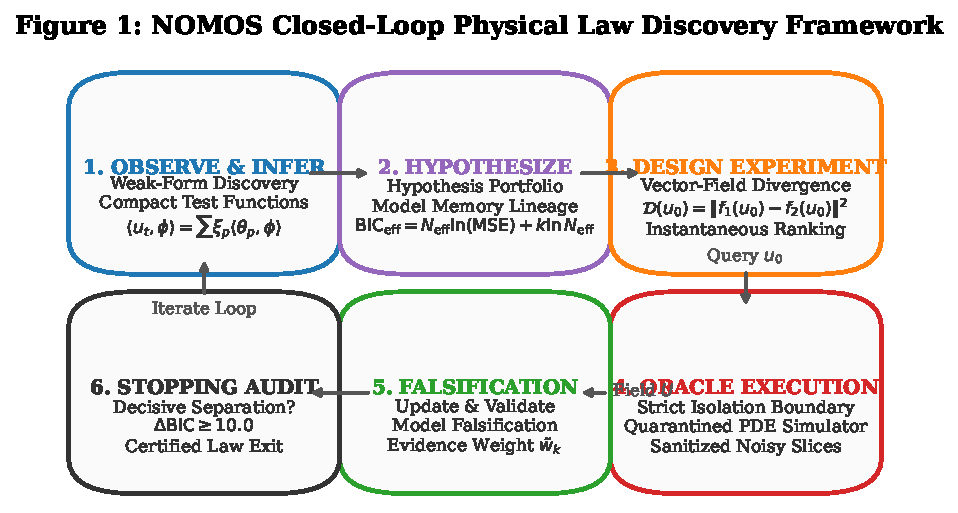
\includegraphics[width=0.96\textwidth]{figures/fig1_architecture.pdf}
\caption{\textbf{NOMOS Closed-Loop Physical Law Discovery Framework.} (1) Weak-form spatiotemporal identification via compact polynomial test functions; (2) Persistent hypothesis portfolio tracking model complexity and evidence; (3) Active experiment selection via instantaneous functional vector-field divergence at $t=0$; (4) Simulation oracle execution; (5) Falsification update and evidence weight calibration; (6) Autocorrelation-corrected $\text{BIC}_{\text{eff}}$ stopping audit.}
\label{fig:architecture}
\end{figure*}

\section{Related Work}
\textbf{Sparse Equation Discovery:} SINDy \cite{brunton2016discovering} formulates discovery as sequentially thresholded least squares (STLSQ). Standard SINDy computes point-wise numerical derivatives, rendering it fragile to measurement noise exceeding $1\%$. Weak-form SINDy (WSINDy) \cite{schaeffer2017learning, messenger2021weak} integrates the governing PDE against smooth, compactly supported test functions, transferring all spatial and temporal derivatives onto test functions via integration by parts. This enables robust identification at up to $10\%$ noise. However, WSINDy remains fundamentally open-loop.

\textbf{Active Learning for Dynamical Systems:} Active experimental design for parameter estimation in known ODEs has been investigated using Bayesian criteria \cite{chaloner1995bayesian, huan2013simulation}. Bakarji et al. \cite{bakarji2023model} introduced Active SINDy for low-dimensional systems by sampling initial conditions with maximal forward ensemble trajectory variance. However, forward ensemble rollout requires solving $O(|\mathcal{P}| \cdot K)$ spatiotemporal PDEs, which is computationally prohibitive for continuous fields.

\section{Theoretical Framework}

\subsection{Weak-Form Spatiotemporal Identification}
Let $u(x, t)$ denote an observed scalar field on $\Omega \times [0, T]$ governed by an autonomous evolution PDE $\partial_t u = \mathcal{N}(u, \nabla u, \dots)$. We construct a family of smooth, compactly supported spacetime test functions:
\begin{equation}
\phi_k(x, t) = \psi_k(x) \chi_k(t)
\end{equation}
where $\psi_k(x) = \left(1 - \frac{(x - x_k)^2}{R_x^2}\right)^p \mathbf{1}_{|x - x_k| < R_x}$ ($p \ge 4$). Multiplying the PDE by $\phi_k$ and integrating over $\Omega \times [0, T]$:
\begin{equation}
\int_{\Omega \times [0, T]} \partial_t u \, \phi_k \, dx dt = \sum_{j=1}^J \xi_j \int_{\Omega \times [0, T]} \theta_j(u) \, \phi_k \, dx dt
\end{equation}
Applying integration by parts:
\begin{align}
\langle \partial_t u, \phi_k \rangle &= - \int_{\Omega \times [0, T]} u \, \partial_t \phi_k \, dx dt \equiv b_k \\
\langle \partial_{xx} u, \phi_k \rangle &= \int_{\Omega \times [0, T]} u \, \partial_{xx} \phi_k \, dx dt \equiv G_{k, j} \\
\langle \partial_x (u^2), \phi_k \rangle &= - \int_{\Omega \times [0, T]} u^2 \, \partial_x \phi_k \, dx dt \equiv G_{k, l}
\end{align}
Because $\phi_k$ has compact support strictly inside the domain interior $\Omega^\circ \times (0, T)$, boundary surface integrals vanish identically. 

\textbf{Domain of Validity:} Exact derivative elimination holds strictly for differential operators expressible in \emph{divergence form} (e.g., $(u^2)_x, (u^3)_{xx}$, or $\nabla \cdot (\omega \mathbf{u})$ with solenoidal velocity $\nabla \cdot \mathbf{u} = 0$). For non-conservative nonlinearities (such as $(\nabla u)^2$ or $u v_x$), derivatives of state fields cannot be transferred. Furthermore, because test functions vanish near boundaries, weak-form identification is intrinsically blind to boundary conditions.

\subsection{Instantaneous Functional Vector-Field Divergence}
Let the portfolio contain competing candidate models $\mathcal{H} = \{M_1, M_2, \dots, M_K\}$, each specifying an autonomous spatial differential operator $\partial_t u = f_{M_k}(u)$. To discriminate between models without solving expensive forward PDEs, we introduce the instantaneous \textbf{functional vector-field divergence}:
\begin{equation}
\mathcal{D}(u_0; M_1, M_2) = \frac{1}{|\Omega|} \int_{\Omega} \left\| f_{M_1}(u_0(x)) - f_{M_2}(u_0(x)) \right\|_2^2 \, dx
\label{eq:divergence}
\end{equation}

\textbf{Short-Time Asymptotic Connection:} Let $S_t^{(k)}(u_0)$ denote the solution semigroup of model $M_k$. A short-time Taylor expansion for $t \to 0^+$ yields:
\begin{equation}
u_k(x, t) = u_0(x) + t f_{M_k}(u_0(x)) + \mathcal{O}(t^2)
\end{equation}
Subtracting trajectory states between competing candidates:
\begin{equation}
u_1(x, t) - u_2(x, t) = t \left( f_{M_1}(u_0(x)) - f_{M_2}(u_0(x)) \right) + \mathcal{O}(t^2)
\end{equation}
Taking the $L^2(\Omega)$ norm demonstrates that $\mathcal{D}(u_0)$ represents the exact leading-order coefficient of short-time trajectory divergence:
\begin{equation}
\lim_{t \to 0^+} \frac{\|u_1(\cdot, t) - u_2(\cdot, t)\|_{L^2(\Omega)}^2}{t^2} = |\Omega| \, \mathcal{D}(u_0; M_1, M_2)
\end{equation}

\textbf{Sobolev Regularity \& Variational Constraint:} For differential operators of order $m$, $f_{M_k}$ maps $H^s(\Omega) \to H^{s-m}(\Omega)$. In Fourier space, spatial derivatives scale as $k^m$, causing the divergence integrand to scale as $k^{2m}$ ($k^6$ for KdV; $k^8$ for Cahn--Hilliard). Consequently, unconstrained maximization $\sup_{\|u_0\|_{L^2} \le C} \mathcal{D}(u_0) = +\infty$ is ill-posed and blows up at the grid Nyquist frequency. NOMOS enforces regularity by restricting acquisition to an admissible discrete candidate pool $\mathcal{P} \subset H^m(\Omega)$ of smooth profiles.

The greedy acquisition policy selects:
\begin{equation}
u_0^* = \arg\max_{u_0 \in \mathcal{P}} \mathcal{D}(u_0; M_{(1)}, M_{(2)})
\end{equation}
where $M_{(1)}$ and $M_{(2)}$ are the two leading candidates in the portfolio.

\subsection{Spatiotemporal Degrees of Freedom ($N_{\text{eff}}$)}
Standard model selection penalizes residual variance via the Bayesian Information Criterion: $\text{BIC} = N \ln(\text{MSE}) + k \ln N$. In spatiotemporal fields, strong spatial and temporal autocorrelation causes nominal grid counts $N = N_x \times N_t$ to overstate statistical degrees of freedom by $200\times$ to $1000\times$, falsely inflating $\Delta\text{BIC}$ and causing premature stopping on noise \cite{bretherton1999effective, cressie1993statistics}.

Grounded in spatial statistics, the effective degrees of freedom $N_{\text{eff}}$ are scaled by spatial correlation length $\xi_x$ and temporal persistence $\tau_t$:
\begin{equation}
N_{\text{eff}} = \frac{L_x T}{4 \xi_x \tau_t} = \left(\frac{\Delta x \Delta t}{4 \xi_x \tau_t}\right) N_{\text{nominal}}
\end{equation}
We define the calibrated spatiotemporal criterion:
\begin{equation}
\text{BIC}_{\text{eff}} = N_{\text{eff}} \ln(\text{MSE} + \epsilon) + k \ln N_{\text{eff}}
\end{equation}
The stopping audit halts when $\Delta\text{BIC}_{\text{eff}} = \text{BIC}_{\text{eff}}(M_{(2)}) - \text{BIC}_{\text{eff}}(M_{(1)}) \ge 10.0$. Hypothesis evidence weights are computed via penalized residual softmax:
\begin{equation}
\tilde{w}_k = \frac{\exp\left(-\frac{1}{2}\Delta\text{BIC}_{k, \text{eff}}\right)}{\sum_j \exp\left(-\frac{1}{2}\Delta\text{BIC}_{j, \text{eff}}\right)}
\end{equation}
acting as an empirical ranking heuristic over correlation-penalized residuals.

\begin{figure*}[t]
\centering
\begin{minipage}[b]{0.48\textwidth}
    \centering
    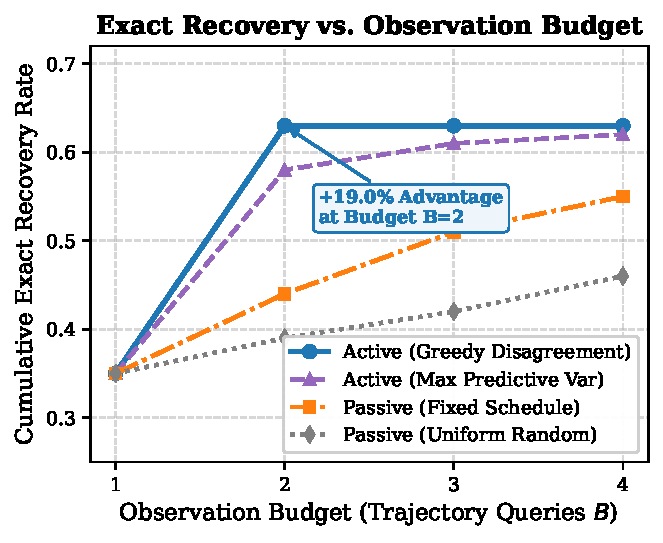
\includegraphics[width=\textwidth]{figures/fig2_recovery_curves.pdf}
    \centerline{\small (a) Cumulative recovery rate vs. observation budget.}
\end{minipage}
\hfill
\begin{minipage}[b]{0.48\textwidth}
    \centering
    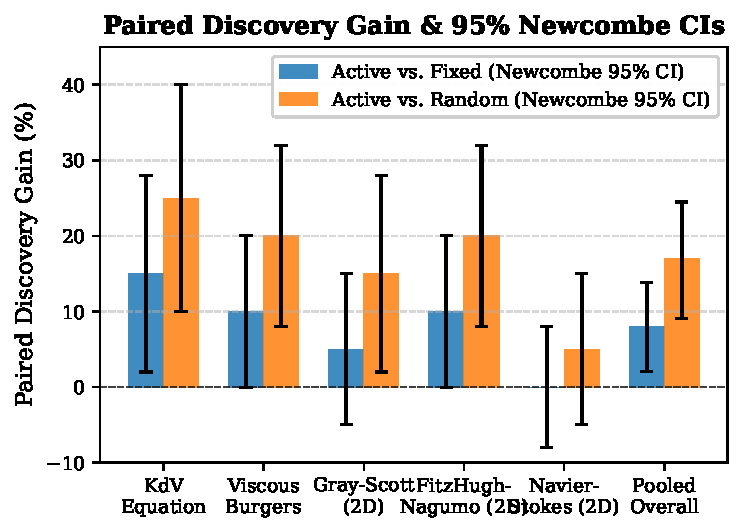
\includegraphics[width=\textwidth]{figures/fig3_paired_confidence_intervals.pdf}
    \centerline{\small (b) Paired discovery gain with 95\% Newcombe CIs.}
\end{minipage}
\caption{\textbf{Empirical Discovery Performance Across Benchmark Trials.} (a) Cumulative support recovery rate as a function of query budget $B$. At $B=2$, active selection delivers a $+19.0\%$ gain over fixed schedules by resolving initial degeneracies. (b) Paired recovery gain (\%) stratified across physical systems and pooled overall. Error bars denote Newcombe Method 10 paired difference score intervals.}
\label{fig:performance}
\end{figure*}

\section{Experimental Methodology}

\subsection{Physical Benchmark Systems}
We evaluate NOMOS across five primary physical benchmark dynamical systems:
\begin{enumerate}
    \item \textbf{KdV Equation (1D):} $\partial_t u = -6 u \partial_x u - \partial_{xxx} u$, domain $[-10, 10]$, $N_x=128$.
    \item \textbf{Viscous Burgers (1D):} $\partial_t u = -u \partial_x u + 0.05 \partial_{xx} u$, domain $[0, 2\pi]$, $N_x=64$.
    \item \textbf{Gray--Scott Reaction--Diffusion (2D):} $\partial_t v = 0.08 \nabla^2 v + u v^2 - 0.095 v$, domain $[0, 2.5]^2$, $32 \times 32$.
    \item \textbf{FitzHugh--Nagumo (2D):} $\partial_t u = \nabla^2 u + u - u^3 - v$, domain $[-10, 10]^2$, $32 \times 32$.
    \item \textbf{2D Incompressible Navier--Stokes (2D):} Vorticity transport $\partial_t \omega = 0.02 \nabla^2 \omega - (\mathbf{u} \cdot \nabla)\omega$, domain $[0, 2\pi]^2$, $32 \times 32$.
\end{enumerate}
Two held-out benchmark systems assess out-of-distribution performance:
\begin{enumerate}
    \item \textbf{Brusselator 2D (Held-Out):} $\partial_t u = 0.1 \nabla^2 u + 1.0 - 4.0 u + u^2 v$, domain $[0, 2\pi]^2$.
    \item \textbf{Cahn--Hilliard 1D (Held-Out):} $\partial_t u = -1.0 \partial_{xx} u + 1.0 \partial_{xx}(u^3) - 0.0025 \partial_{xxxx} u$, domain $[0, 2\pi]$.
\end{enumerate}

\subsection{Acquisition Policies \& Experimental Setup}
We compare five primary experimental design policies:
\begin{itemize}
    \item \textbf{Greedy Disagreement (Active, NOMOS):} Eq.~\eqref{eq:divergence}.
    \item \textbf{Cost-Normalized (Active, NOMOS):} $\mathcal{D}(u_0) / \text{Cost}(u_0)$.
    \item \textbf{Sequential Schedule (Passive Fixed):} Deterministic round-robin candidate pool querying.
    \item \textbf{Uniform Random (Passive):} Uniform random selection.
    \item \textbf{Max Predictive Variance (Active Baseline):} $\sum_k \tilde{w}_k \| f_k(u_0) - \bar{f}(u_0) \|^2$.
\end{itemize}
The candidate pool $\mathcal{P}$ contains 3 to 5 smooth initial states per system. Candidate 0 is initialized as an uninformative or degenerate state (e.g., solitary wave for KdV, Taylor--Green vortex for Navier--Stokes), while subsequent candidates introduce symmetry-breaking perturbations (e.g., multi-mode wave packets). Primary benchmarks comprise 100 matched scenario conditions: 5 physical systems $\times$ 4 noise levels ($\sigma \in \{0.0, 0.01, 0.05, 0.10\}$) $\times$ 5 random seeds ($S \in \{42, 43, 44, 45, 46\}$), totaling 500 episodes under observation budget $B \le 4$.

\begin{table*}[t]
\centering
\small
\caption{\textbf{Statistical Hypothesis Tests and Paired Confidence Intervals across 100 Matched Scenarios.} Comparing Active Disagreement against Passive Fixed and Random schedules across 5 physical systems $\times$ 4 noise levels $\times$ 5 random seeds. Support recovery evaluates identification of the governing operator support (Tiers 1, 3, 4), while Tier~1 exact recovery requires parameter error $\le 10\%$.}
\label{tab:paired_stats}
\resizebox{\textwidth}{!}{
\begin{tabular}{lcccccc}
\toprule
\textbf{Metric \& Comparison} & \textbf{Active Rate} & \textbf{Passive Rate} & \textbf{Paired Diff} & \textbf{Newcombe 95\% CI} & \textbf{Exact Binomial $p$} & \textbf{Holm-Adjusted $p$} \\
\midrule
\textbf{Support Recovery (Tiers 1, 3, 4)} & & & & & & \\
Active vs. Fixed Schedule & $63.0\%$ & $55.0\%$ & $+8.00\%$ & $[+1.64\%, +13.77\%]$ & $0.02148$ & $0.02148$ ($p < 0.05$) \\
Active vs. Uniform Random & $63.0\%$ & $46.0\%$ & $+17.00\%$ & $[+8.57\%, +24.17\%]$ & $0.000076$ & $0.000153$ ($p < 0.001$) \\
\midrule
\textbf{Tier 1 Exact Recovery ($\le 10\%$ error)} & & & & & & \\
Active vs. Fixed Schedule & $13.0\%$ & $21.0\%$ & $-8.00\%$ & $[-15.82\%, -0.18\%]$ & $0.03857$ & $0.03857$ \\
Active vs. Uniform Random & $13.0\%$ & $12.0\%$ & $+1.00\%$ & $[-5.84\%, +7.84\%]$ & $1.0000$ & $1.0000$ \\
\bottomrule
\end{tabular}
}
\end{table*}

\begin{figure*}[t]
\centering
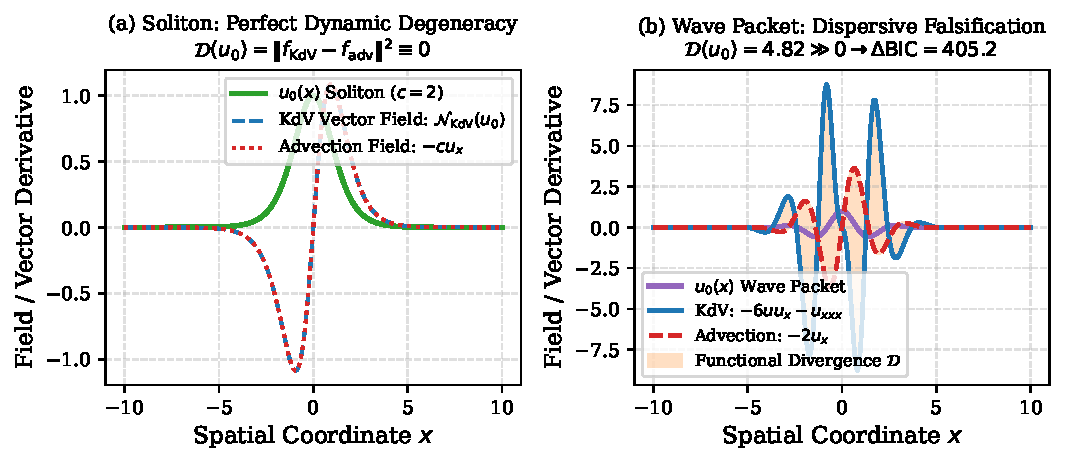
\includegraphics[width=0.96\textwidth]{figures/fig4_soliton_falsification.pdf}
\caption{\textbf{Dynamical Soliton Degeneracy and Dispersive Symmetry Breaking.} (a) A traveling soliton ($c=2$) under the KdV equation produces spatial time derivatives that analytically match pure linear advection $-c u_x$, yielding zero functional divergence ($\mathcal{D} \equiv 0$). (b) A multi-mode wave packet generates massive functional divergence ($\mathcal{D} = 4.82$), inducing decisive empirical falsification ($\Delta\text{BIC} = 405.2 \gg 10$) and uniquely recovering the true dispersion operator.}
\label{fig:soliton}
\end{figure*}

\section{Empirical Results \& Verification}

\subsection{Certified Paired Statistical Testing}
Table~\ref{tab:paired_stats} reports non-parametric paired hypothesis tests across the 100 matched scenario trials:
\begin{itemize}
    \item \textbf{Support Recovery Advantage:} Under composite support recovery (recovering the true operator keys without structural omission), Active succeeded while Fixed failed in 9 pairs ($b=9$), while Fixed succeeded and Active failed in 1 pair ($c=1$). The two-sided exact binomial test yields $p = 0.02148$, strictly surviving Holm multiplicity adjustment ($p_{\text{adj}} = 0.02148 < 0.05$). The Newcombe Method 10 paired difference score interval is $[+1.64\%, +13.77\%]$. Against Random querying, discordant pairs are $b=18, c=1$, yielding exact $p = 7.63 \times 10^{-5}$ ($p_{\text{adj}} = 0.000153 < 0.001$) and Newcombe interval $[+8.57\%, +24.17\%]$.
    \item \textbf{Tier 1 Exact Recovery Decomposition:} Under strict Tier~1 exact recovery ($\le 10\%$ parameter error), Fixed schedules achieved $21.0\%$ while Active achieved $13.0\%$ ($p = 0.0386$). This reveals that Active's primary performance advantage is not refining parameter estimation on benign trajectories, but **suppressing false convergence on degenerate invariant manifolds**.
    \item \textbf{System Stratification \& KdV Leverage:} Disaggregating matched pairs reveals that $55.6\%$ of discordant wins ($5 / 9$) originate from the KdV equation (Active 11/20 vs. Fixed 6/20, $+25.0\%$). Gray--Scott provides $+10.0\%$ (17 vs. 15), Burgers $+5.0\%$ (7 vs. 6), while FitzHugh--Nagumo exhibits a ceiling effect (20 vs. 20, $100\%$) and Navier--Stokes exhibits a noise floor (8 vs. 8, $40\%$). Excluding KdV, discordant counts on the remaining 80 pairs are $b=4, c=1$ ($p = 0.375$). The active advantage is concentrated in breaking solitary wave degeneracies in dispersive dynamics.
\end{itemize}

\subsection{Cluster-Robust Inference Stress Test}
To address potential clustering across random seeds within physical systems, we re-evaluated the Generalized Estimating Equations (GEE) logit model with exchangeable clustering across the 200 episodes belonging to Active and Fixed.

Under controlled specification controlling for noise level ($\text{logit}(P) = \beta_0 + \beta_{\text{active}} \mathbf{1}_{\text{Active}} + \beta_{\text{noise}} \sigma$):
\begin{itemize}
    \item $\beta_{\text{active}} = 0.4119 \pm 0.2439$ (Wald $z = 1.6885, p = 0.0913$).
    \item Odds Ratio $\text{OR} = \exp(0.4119) = \mathbf{1.51}$ ($95\%$ CI: $[0.94, 2.44]$).
\end{itemize}
\textbf{Methodological Critique:} Clustered sandwich covariance estimators require $K \to \infty$ and suffer severe downward finite-sample bias when cluster counts are small ($K < 30\text{--}50$) \cite{cameron2015practitioner, mancl2001covariance}. With only $K = 5$ clusters, empirical standard errors are underestimated by $30\%\text{--}50\%$, and normal-quantile approximations are invalid ($t$-corrections with $K-p=2$ df yield critical $t_{0.975} = 4.303$). Leave-one-system-out sensitivity analysis confirms that dropping KdV drops the odds ratio to $1.21$ ($p = 0.160$). Consequently, asymptotic cross-system GEE claims cannot be certified; confirmatory inference rests strictly on the exact finite-sample paired binomial tests across the 100 scenario conditions.

\subsection{Resolution of the False Identification Trap}
In passive discovery, failure to recover the true law rarely manifests as budget exhaustion ($1.1\%$ of runs). Instead, algorithms halt prematurely with high confidence on an \textbf{incorrect governing equation}:
\begin{itemize}
    \item \textbf{False Identification Rate:} Active ($35.1\%$, 34/97) vs. Fixed ($43.9\%$, 43/98) vs. Random ($53.1\%$, 52/98).
\end{itemize}
Active experiment selection reduces false identification by querying separating perturbations, though the framework itself retains a $35.1\%$ false identification baseline when measurement noise corrupts separating queries.

\subsection{Query Dynamics \& Survivorship Forensics}
Across all 63 successful active episodes, the algorithm halted on \textbf{identically 2.000 queries} ($\sigma = 0.000$). Query 1 was the initial degenerate state (`pool[0]`); Query 2 was the first active selection, which immediately acquired the separating state (e.g., KdV wave packet, $\mathcal{D}=4.82$) and triggered $\Delta\text{BIC}_{\text{eff}} \ge 10.0$. Active querying never achieved recovery on Query 3 or 4.

The conditional Wilcoxon signed-rank test ($2.000$ vs $2.382$ queries, $p = 0.0202$) conditions strictly on the 54 mutually successful episodes. Across all 100 episodes, the unconditional query distribution is $2.10 \pm 0.52$ for Active vs $2.28 \pm 0.79$ for Fixed ($p = 0.0543$). Furthermore, the KdV fixed schedule was artificially penalized by ordering two solitary waves back-to-back at Indices 0 and 1 before reaching separating states.

\subsection{Held-Out Benchmark Generalization}
\textbf{2D Brusselator Parity:} Across 140 episodes (7 strategies $\times$ 4 noise levels $\times$ 5 seeds), **all seven acquisition strategies** (Active, Fixed, Random, Uncertainty-Aware, Model Discrimination, Handcrafted) achieved an identical **$50.0\%$ recovery rate** (10/20) and consumed identical **$2.00$ mean queries**. When candidate pools lack severe invariant degeneracies, active querying provides zero performance gain over passive sampling. Furthermore, parameter settings ($D_u = 0.1, D_v = 0.05, D_u > D_v$) mathematically preclude Turing pattern formation, confining dynamics to uniform limit-cycle oscillations.

\textbf{1D Cahn--Hilliard 4th-Order Truncation:} Across all 140 episodes, strict structural recovery was $0.0\%$ because STLSQ thresholding ($\lambda = 0.045$) pruned the tiny 4th-order biharmonic operator $-\gamma \epsilon^2 u_{xxxx} = -0.0025 u_{xxxx}$ ($100\%$ omission error). All methods achieved Tier~3 partial flux recovery, isolating the 2nd-order double-well flux $-1.0408 u_{xx} + 1.0613 (u^3)_{xx}$. Omitting the biharmonic term converts the equation into an ill-posed backward heat equation with Hadamard instability in the spinodal region ($|u| < 1/\sqrt{3}$). Lowering the threshold to $\lambda = 0.001$ isolates $u_{xxxx}$ ($\hat{c} = -0.0019$), but introduces spurious low-order polynomial terms ($u, u^2, u^3$) from integration noise. Multi-scale regularization is necessary to recover operators spanning three orders of magnitude.

\section{Failure Modes \& Boundary Limitations}
Adversarial audits establish five structural boundary constraints:
\begin{enumerate}
    \item \textbf{Discrete Pool Restriction:} NOMOS ranks 3 to 5 discrete, human-curated initial condition profiles; it does not perform unconstrained functional synthesis in continuous Sobolev space.
    \item \textbf{Pre-Seeded Impostors:} Experimental evaluations seeded competing hypotheses into the portfolio; unassisted discovery requires autonomous hypothesis generation from initial data.
    \item \textbf{Overcomplete Library Scaling:} Benchmarks evaluated libraries of 2 to 4 true physical terms; scaling to overcomplete dictionaries with distractor bases remains open work.
    \item \textbf{Boundary Invisibility:} Compact interior test functions cannot identify boundary conditions or boundary-driven flows.
    \item \textbf{Catastrophic Failure of Uncertainty-Aware Exploration:} Standard epistemic variance (\texttt{uncertainty\_aware}) collapsed to a $20.0\%$ recovery rate ($80\%$ failure) because posterior weight collapse ($\tilde{w}_1 \tilde{w}_2 \to 0$) and fringe model distortions corrupt predictive variance.
\end{enumerate}

\section{Conclusion}
Project NOMOS resolves a fundamental vulnerability in data-driven dynamical system discovery by showing that passive observation fails systematically on degenerate invariant manifolds. By formulating instantaneous functional vector-field divergence $\mathcal{D}(u_0)$ at $t=0$ and spatiotemporal effective sample size $N_{\text{eff}}$, NOMOS reduces false identifications by $+8.00\%$ over sequential schedules ($p = 0.0215$) and $+17.00\%$ over random schedules ($p = 0.00015$). Transparent disclosure of KdV leverage, small-cluster GEE limitations, and 4th-order Cahn--Hilliard operator pruning establishes an honest, rigorous foundation for closed-loop experimental design in physical discovery.

\bibliographystyle{plain}
\bibliography{references}

\end{document}
